\documentclass[../notes.tex]{subfiles}

\pagestyle{main}
\renewcommand{\chaptermark}[1]{\markboth{\chaptername\ \thechapter\ (#1)}{}}
\stepcounter{chapter}

\begin{document}




\chapter{Templates}
\section{Problem 2}
\begin{itemize}
    \item \marginnote{9/25:}We now begin discussing Problem 2.
    \begin{figure}[h!]
        \centering
        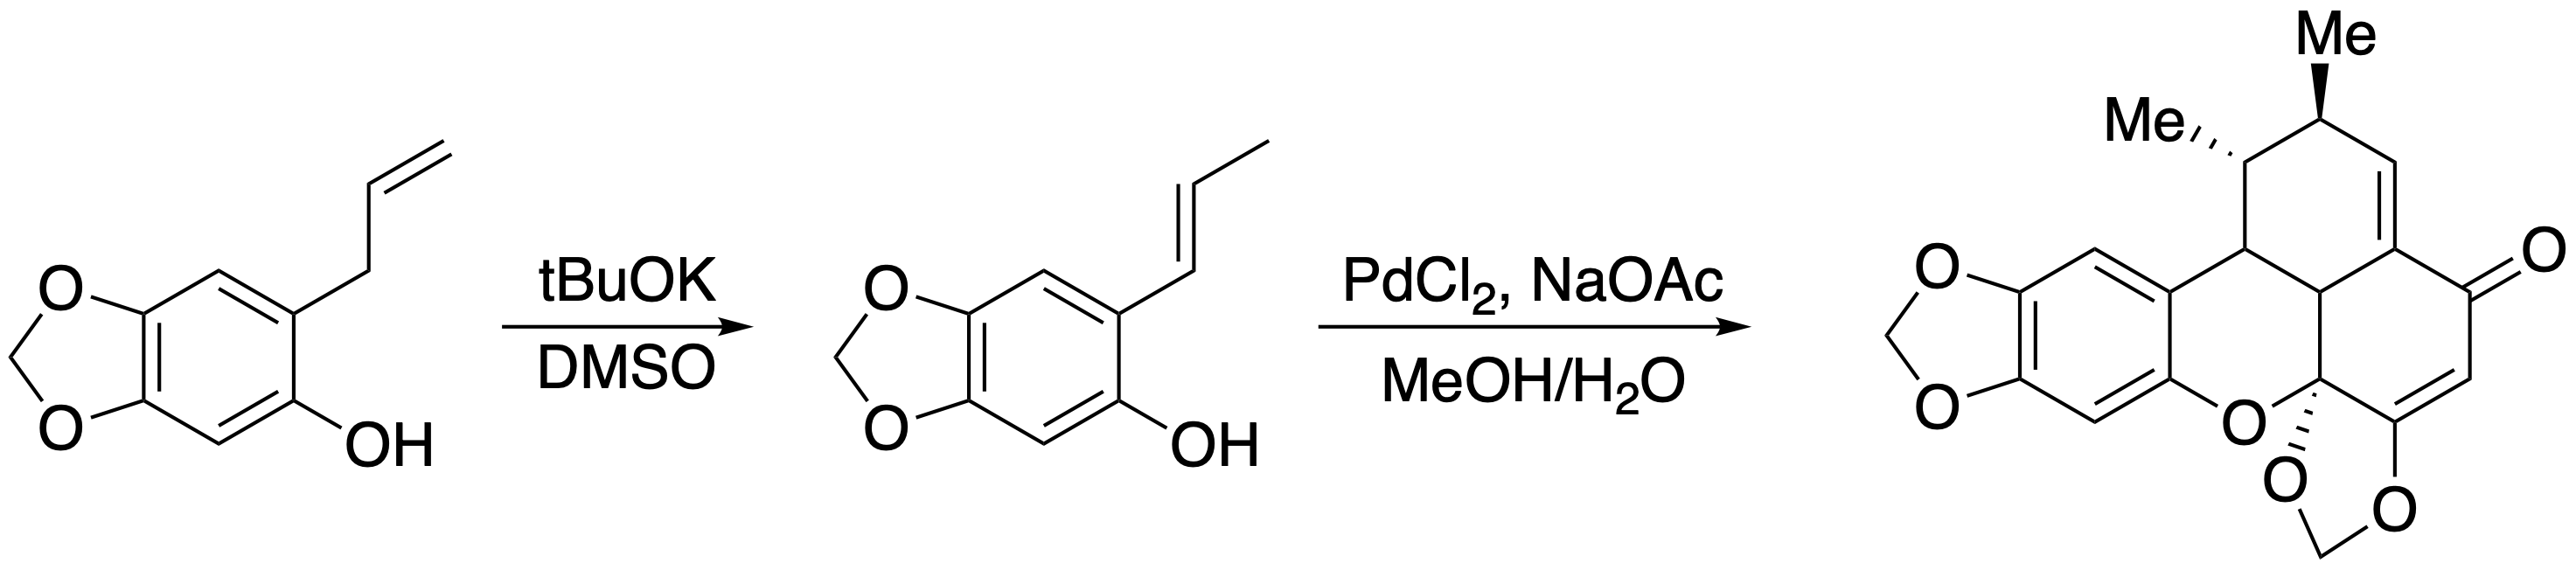
\includegraphics[width=0.8\linewidth]{WPSet2Q2.png}
        \caption{Wendlandt PSet 2, Q2.}
        \label{fig:WPSet2Q2}
    \end{figure}
    \item This is similar to an \textbf{Overman rearrangement}.
    \item Palladium is unlikely to activate the aromatic $\pi$-system --- and if it did, it would do so in an $\eta^6$-fashion. There are better things for it to coordinate to.
    \item A Wacker oxidation is net oxidative, whereas this is a redox neutral reaction.
    \item Palladium is proposed to be a \textbf{template} in this reaction; that is, it is to bring the fragments together.
    \item Frank's proposal is much closer.
    \begin{itemize}
        \item He sees the "latent \emph{ortho}-quinone methide."
        \item Entry into the dimerization steps is by bringing the carbon-carbon backbone together.
    \end{itemize}
    \item In solution, \ce{PdCl2} will get solvated immediately to have two X-type ligands and two L-type ligands, so that part of my proposal was correct.
    \begin{itemize}
        \item \ce{PdCl2(MeOH)2} could then ligand exchange with the substrate, which also has a good L-type ligand and X-type ligand.
        \item Kicking out HCl's will lead to \ce{NaCl} and \ce{HOAc} in basic solution.
    \end{itemize}
    \item Think about the $\pi$-orbitals on the alkene L-ligand that would interact with palladium's $d$-orbitals.
    \item Alkenes really want to be perpendicular to palladium; crystal structures support this.
    \item Altogether, the full solution to PSet 2, Q2 is on the next page.
    \begin{figure}[h!]
        \centering
        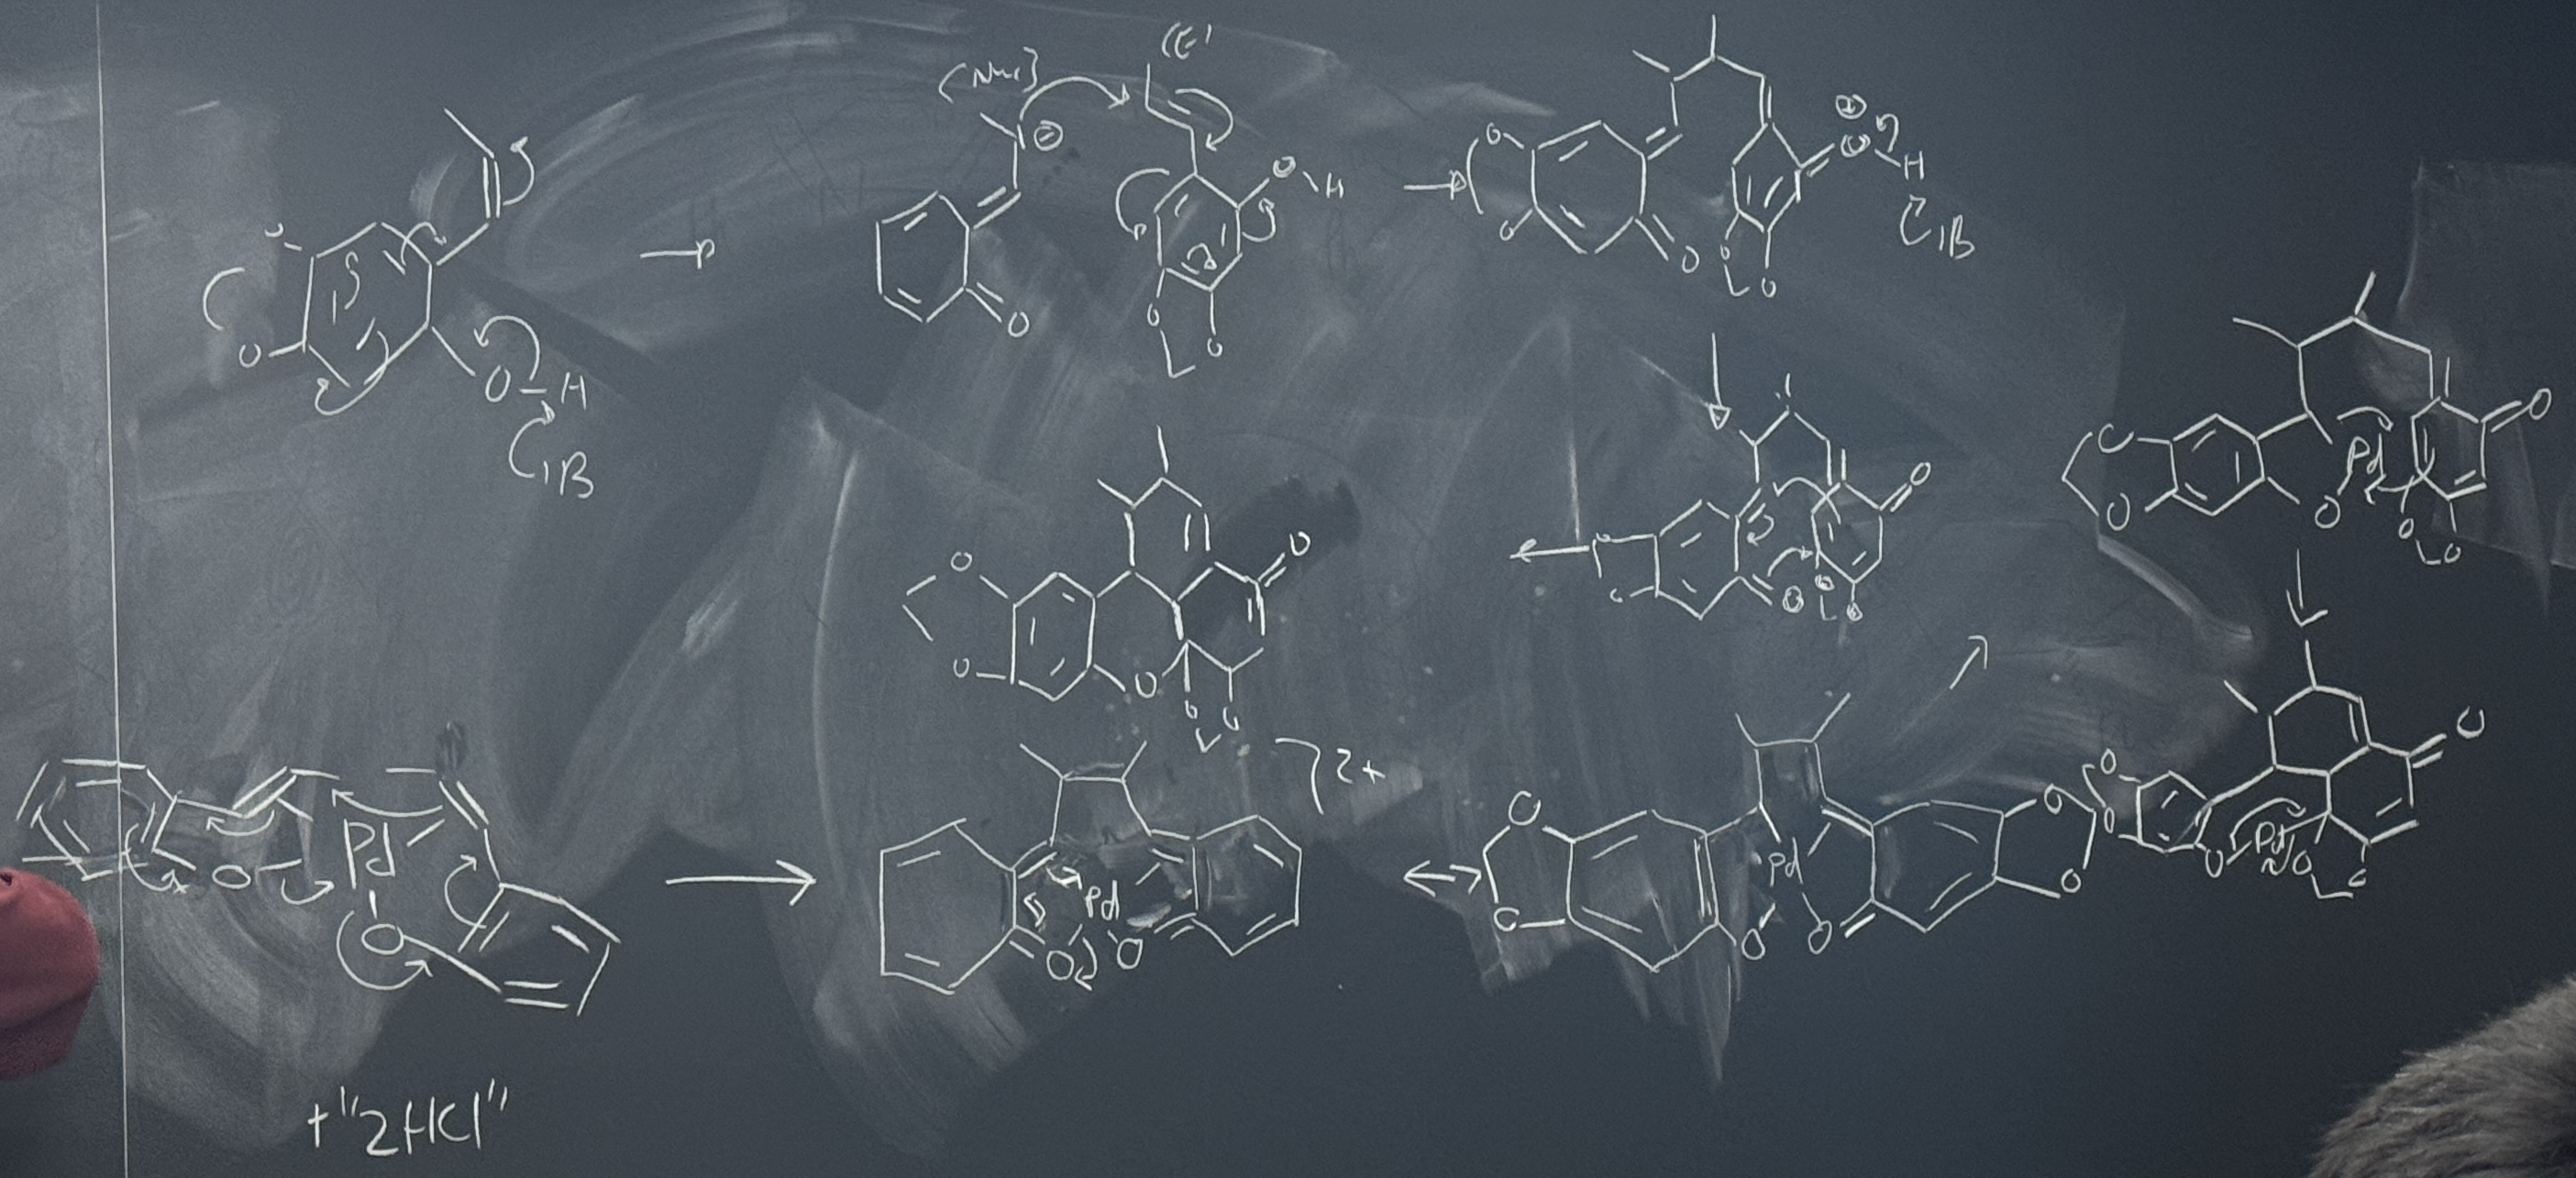
\includegraphics[width=0.8\linewidth]{WPSet2Q2S.JPG}
        \caption{Wendlandt PSet 2, Q2 solution.}
        \label{fig:WPSet2Q2S}
    \end{figure}
\end{itemize}




\end{document}